\paragraph{Mapping $f(x)$ from $GF(2^8)$ to $GF((2^4)^2)$}\mbox{}\\
Output bits of this operation depend on as much as 7 input bits, therefore to make it use only 4-input LUTs it is necessary to split it into two substages (\ref{eg:f-split}) (fig. \ref{fig:f-split}) -- $f_a$ (\ref{eq:mul_delta_a}) and $f_b$ (\ref{eq:mul_delta_b}).

\begin{equation}
\label{eg:f-split}
f(x) = f_b \circ f_a(x)
\end{equation}

\begin{figure}[!h]
\centering
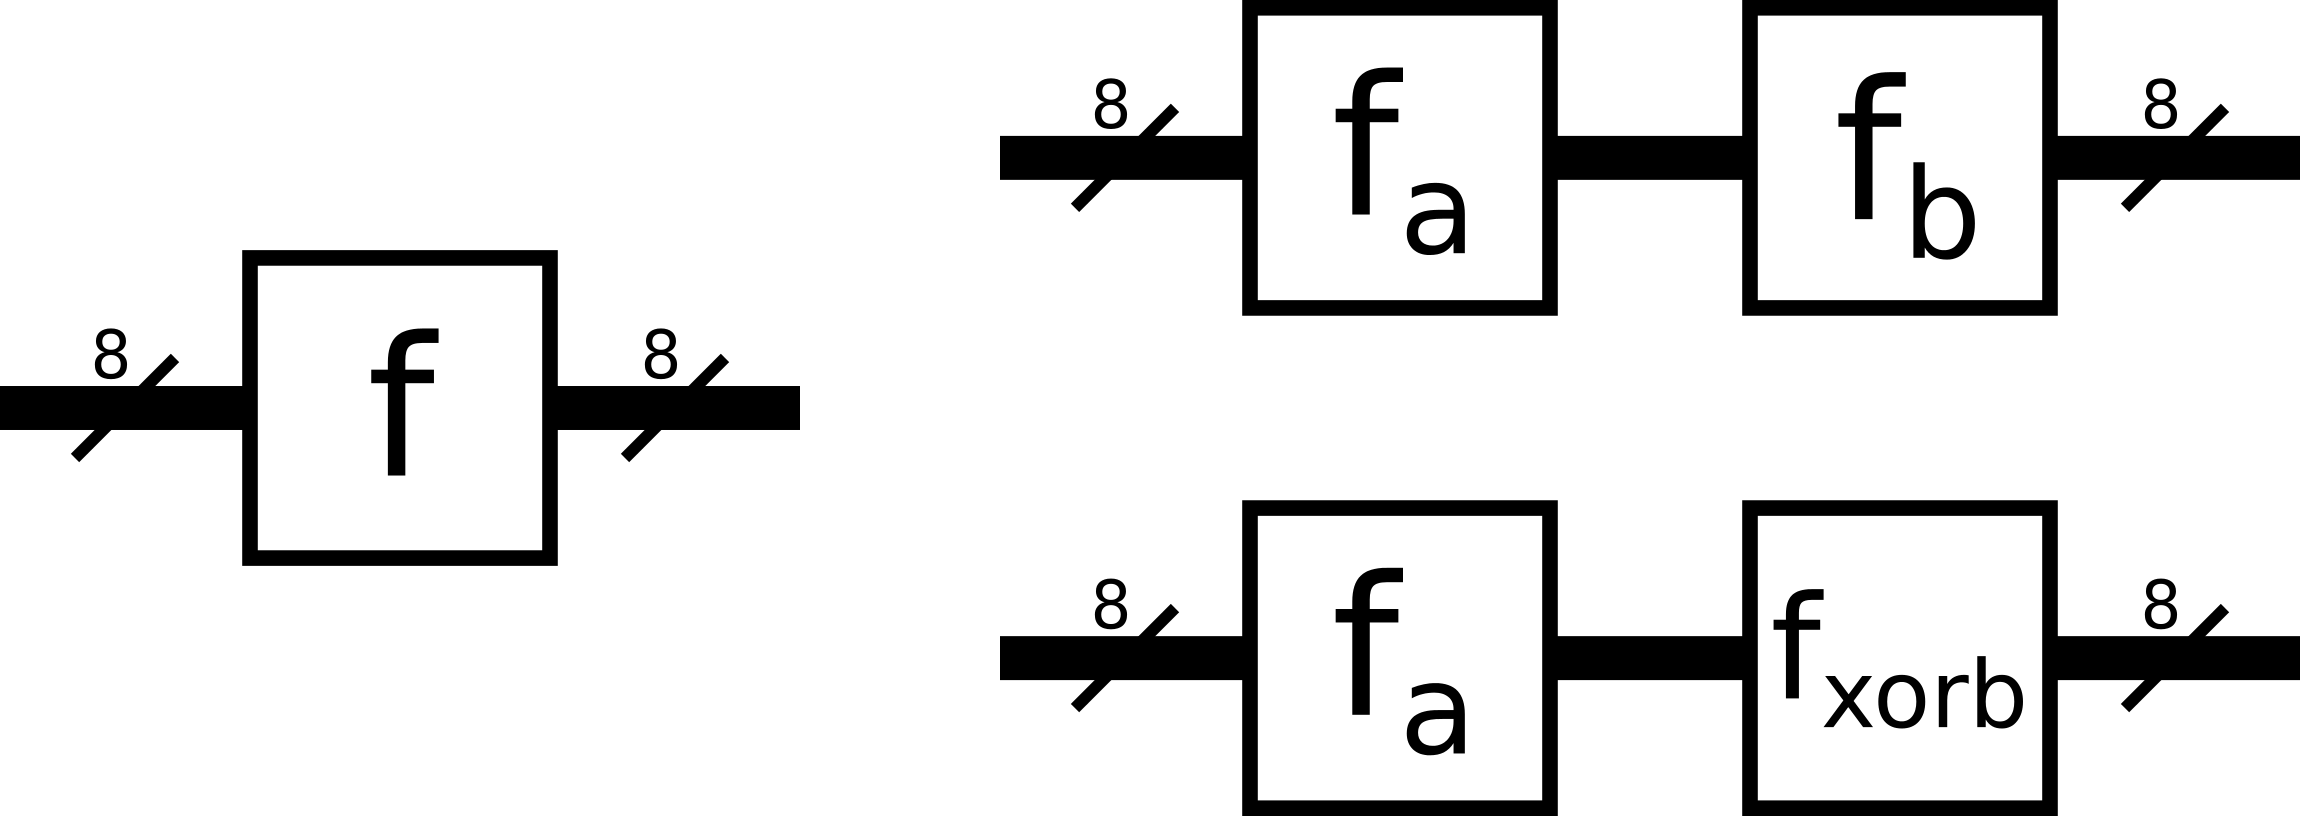
\includegraphics[scale=4]{f-split}
\caption{Decomposition of mapping $f(x)$ from $GF(2^8)$ to $GF((2^4)^2)$ into two stages}
\label{fig:f-split}
\end{figure}

\begin{figure}[!h]
\begin{multicols}{2}

\begin{equation}
\label{eq:mul_delta_a}
\begin{aligned}
b_{a0}    &= b_0                    \\
b_{a1}    &= b_1                    \\
b_{a2}    &= b_2                    \\
b_{a3}    &= b_3                    \\
b_{a4}    &= b_4                    \\
b_{a5}    &= b_5                    \\
b_{a6}    &= b_6                    \\
b_{a7}    &= b_7                    \\
b_{a23}   &= b_2 + b_3              \\
b_{a57}   &= b_5 + b_7              \\
b_{a14}   &= b_1 + b_4                
\end{aligned}
\end{equation}

\break
 
\begin{equation}
\label{eq:mul_delta_b}
\begin{aligned}
b'_0 &= b_{a0} + b_{a1} + b_{a6}           \\
b'_1 &= b_{a6} + b_{a14}                   \\
b'_2 &= b_{a7} + b_{a14} + b_{23}          \\
b'_3 &= b_{a1} + b_{a2} + b_{a6} + b_{a7}  \\
b'_4 &= b_{a1} + b_{a57} + b_{a23}         \\
b'_5 &= b_{a57} + b_{a23}                  \\
b'_6 &= b_{a6} + b_{a7} + b_{a14} + b_{a23}\\
b'_7 &= b_{a57}                            
\end{aligned}
\end{equation}

\end{multicols}
\end{figure}

\newpage
In SubBytes transformation after mapping $f(x)$ from $GF(2^8)$ to $GF((2^4)^2)$ high and low words of the result are xored together (fig. \ref{fig:mul_inv_gf242}). This operation can be performed concurently with $f_b(x)$ mapping to avoid creating a separate stage only for a xor operation.

\begin{equation}
\begin{aligned}
f_{xor}(x) &= f(x)_{low} + f(x)_{high} \\
f_{xor}(x) &= f_{xorb} \circ f_a(x)
\end{aligned}
\end{equation}

\begin{equation}
\label{eq:mul_delta_xor}
\begin{aligned}
b_{xorb0} &= b_{a0} + b_{a23} + b_{a567}       \\
b_{xorb1} &= b_{a1234} + b_{567}               \\
b_{xorb2} &= b_{a6}                            \\
b_{xorb3} &= b_{a1} + b_{a2} + b_{a5} + b_{a6}
\end{aligned}
\end{equation}

From equations (\ref{eq:mul_delta_a}), (\ref{eq:mul_delta_b}) and (\ref{eq:mul_delta_xor}) it is apparent that each stage output bit depends on no more than 4 inputs.




\paragraph{Mapping $f^{-1}(x)$ from $GF((2^4)^2)$ to $GF(2^8)$ combined with AES affine transformation}\mbox{}\\
Analoguously to mapping $f(x)$ from $GF(2^8)$ to $GF((2^4)^2)$, mapping $f^{-1}(x)$ from $GF((2^4)^2)$ to $GF(2^8)$ combined with affine transformation (\ref{sec:comb-theory}) (\ref{eq:fa-split}) (fig. \ref{fig:fa-split}) should be split into two substages --  $f^{-1}_a$ (\ref{eq:mul_delta_inf_a}) and $f^{-1}_b$ (\ref{eq:mul_delta_inf_b}).

\begin{equation}
\label{eq:fa-split}
\begin{aligned}
f^{-1}(x) &= f_b^{-1}(x) \circ f_a^{-1}(x) \\
\end{aligned}
\end{equation}

\begin{figure}[!h]
\centering
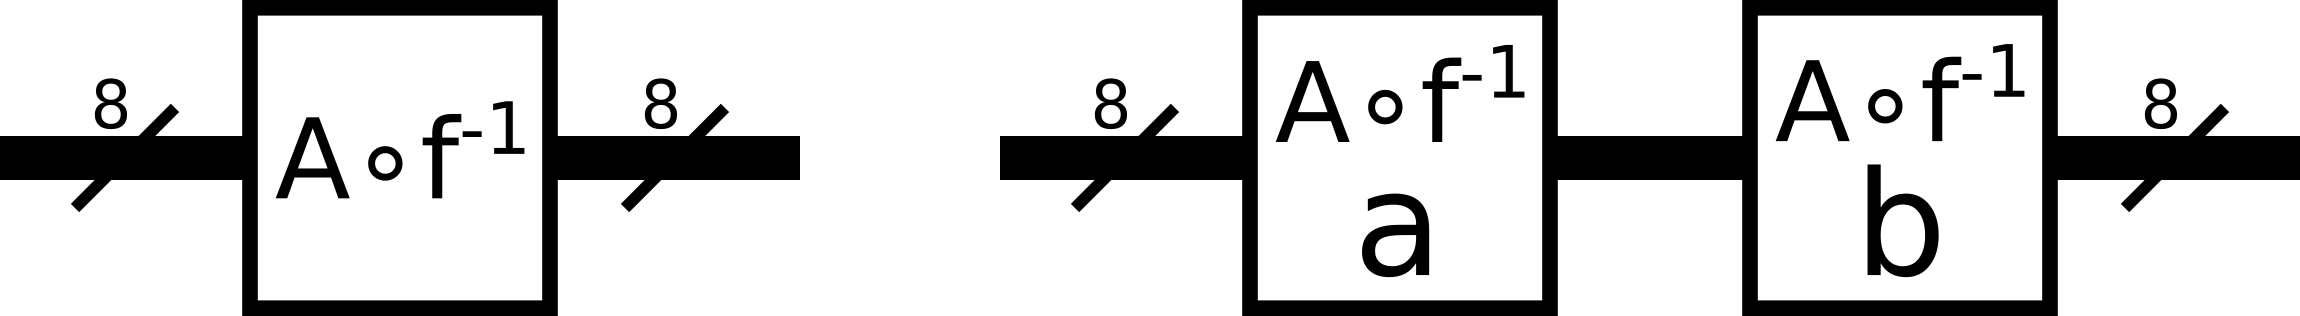
\includegraphics[scale=4]{fa-split}
\caption{Decomposition of mapping $f^{-1}(x)$ from $GF((2^4)^2)$ to $GF(2^8)$ combined with AES affine transformation into two stages}
\label{fig:fa-split}
\end{figure}


\begin{figure}[!h]
\begin{multicols}{2}

\begin{equation}
\label{eq:mul_delta_inf_a}
\begin{aligned}
b_{a0}    &= b_0                    \\
b_{a7}    &= b_7                    \\
b_{a23}   &= b_2 + b_3              \\
b_{a012}  &= b_0 + b_1 + b_2        \\
b_{a023}  &= b_0 + b_2 + b_3        \\
b_{a456}  &= b_4 + b_5 + b_6        \\
b_{a0147} &= b_0 + b_1 + b_4 + b_7  \\
b_{a27N}  &= b_2 + b_7 + 1          \\
b_{a67N}  &= b_6 + b_7 + 1            
\end{aligned}
\end{equation}

\begin{equation}
\label{eq:mul_delta_inf_b}
\begin{aligned}
b'_0 &= b_{a012} + b_{67N}           \\
b'_1 &= b_{a0} + b_{a7} + 1          \\
b'_2 &= b_{a023} + b_{a456}          \\
b'_3 &= b_{a012}                     \\
b'_4 &= b_{a0147}                    \\
b'_5 &= b_{a27N}                     \\
b'_6 &= b_{a456} + b_{a7} + 1        \\
b'_7 &= b_{a23} + b_{a7}                    
\end{aligned}
\end{equation}

\end{multicols}
\end{figure}

From equations (\ref{eq:mul_delta_inf_a}) and (\ref{eq:mul_delta_inf_b}) it is apparent that each stage output bit depends on no more than 4 inputs. Note that $xor$ with $1$ value is merely a $not$ operation, and it does not increase input count. It is also true that all outputs of $f_b^{-1}(x)$ stage depend on no more than 2 inputs, so they can be xored with 2 other independent inputs to form a stage, which is important for a stage in key expansion pipeline.




\paragraph{Multiplicative inversion in $GF(2^4)$}\mbox{}\\
This operation has only 4 inputs, so it is can already be implemented using a 4-input LUT.

\paragraph{Multiplication by constant $\phi$ in $GF(2^2)$}\mbox{}\\
This operation has only 2 inputs, so it is can already be implemented using a 4-input LUT. 

\paragraph{Multiplication by constant $\lambda$ in $GF(2^4)$}\mbox{}\\
This operation has only 4 inputs, so it is can already be implemented using a 4-input LUT. Moreover, it is only used as part of SubBytes transformation directly after squaring in $GF(2^4)$. Because squaring takes only 4 inputs, and multiplication by $\lambda$ operates only on output of squaring, those two operations can be combined into single stage. Such merging only increases length of critical path of the stage (which is irrelevant) but does not increase number of inputs, which is still 4.


\paragraph{Multiplication in $GF(2^2)$}\mbox{}\\
This operation has only 4 inputs, so it is can already be implemented using a 4-input LUT. Every output depends on at most 3 inputs, so it is possible to xor each of them with a signal that does not depend on anything (was just registered).

\paragraph{Multiplication in $GF(2^4)$}\mbox{}\\
This operation has 8 inputs, so it is necessary to split it into two stages (fig. \ref{fig:mul-gf4-split}).

\begin{figure}[!h]
\centering
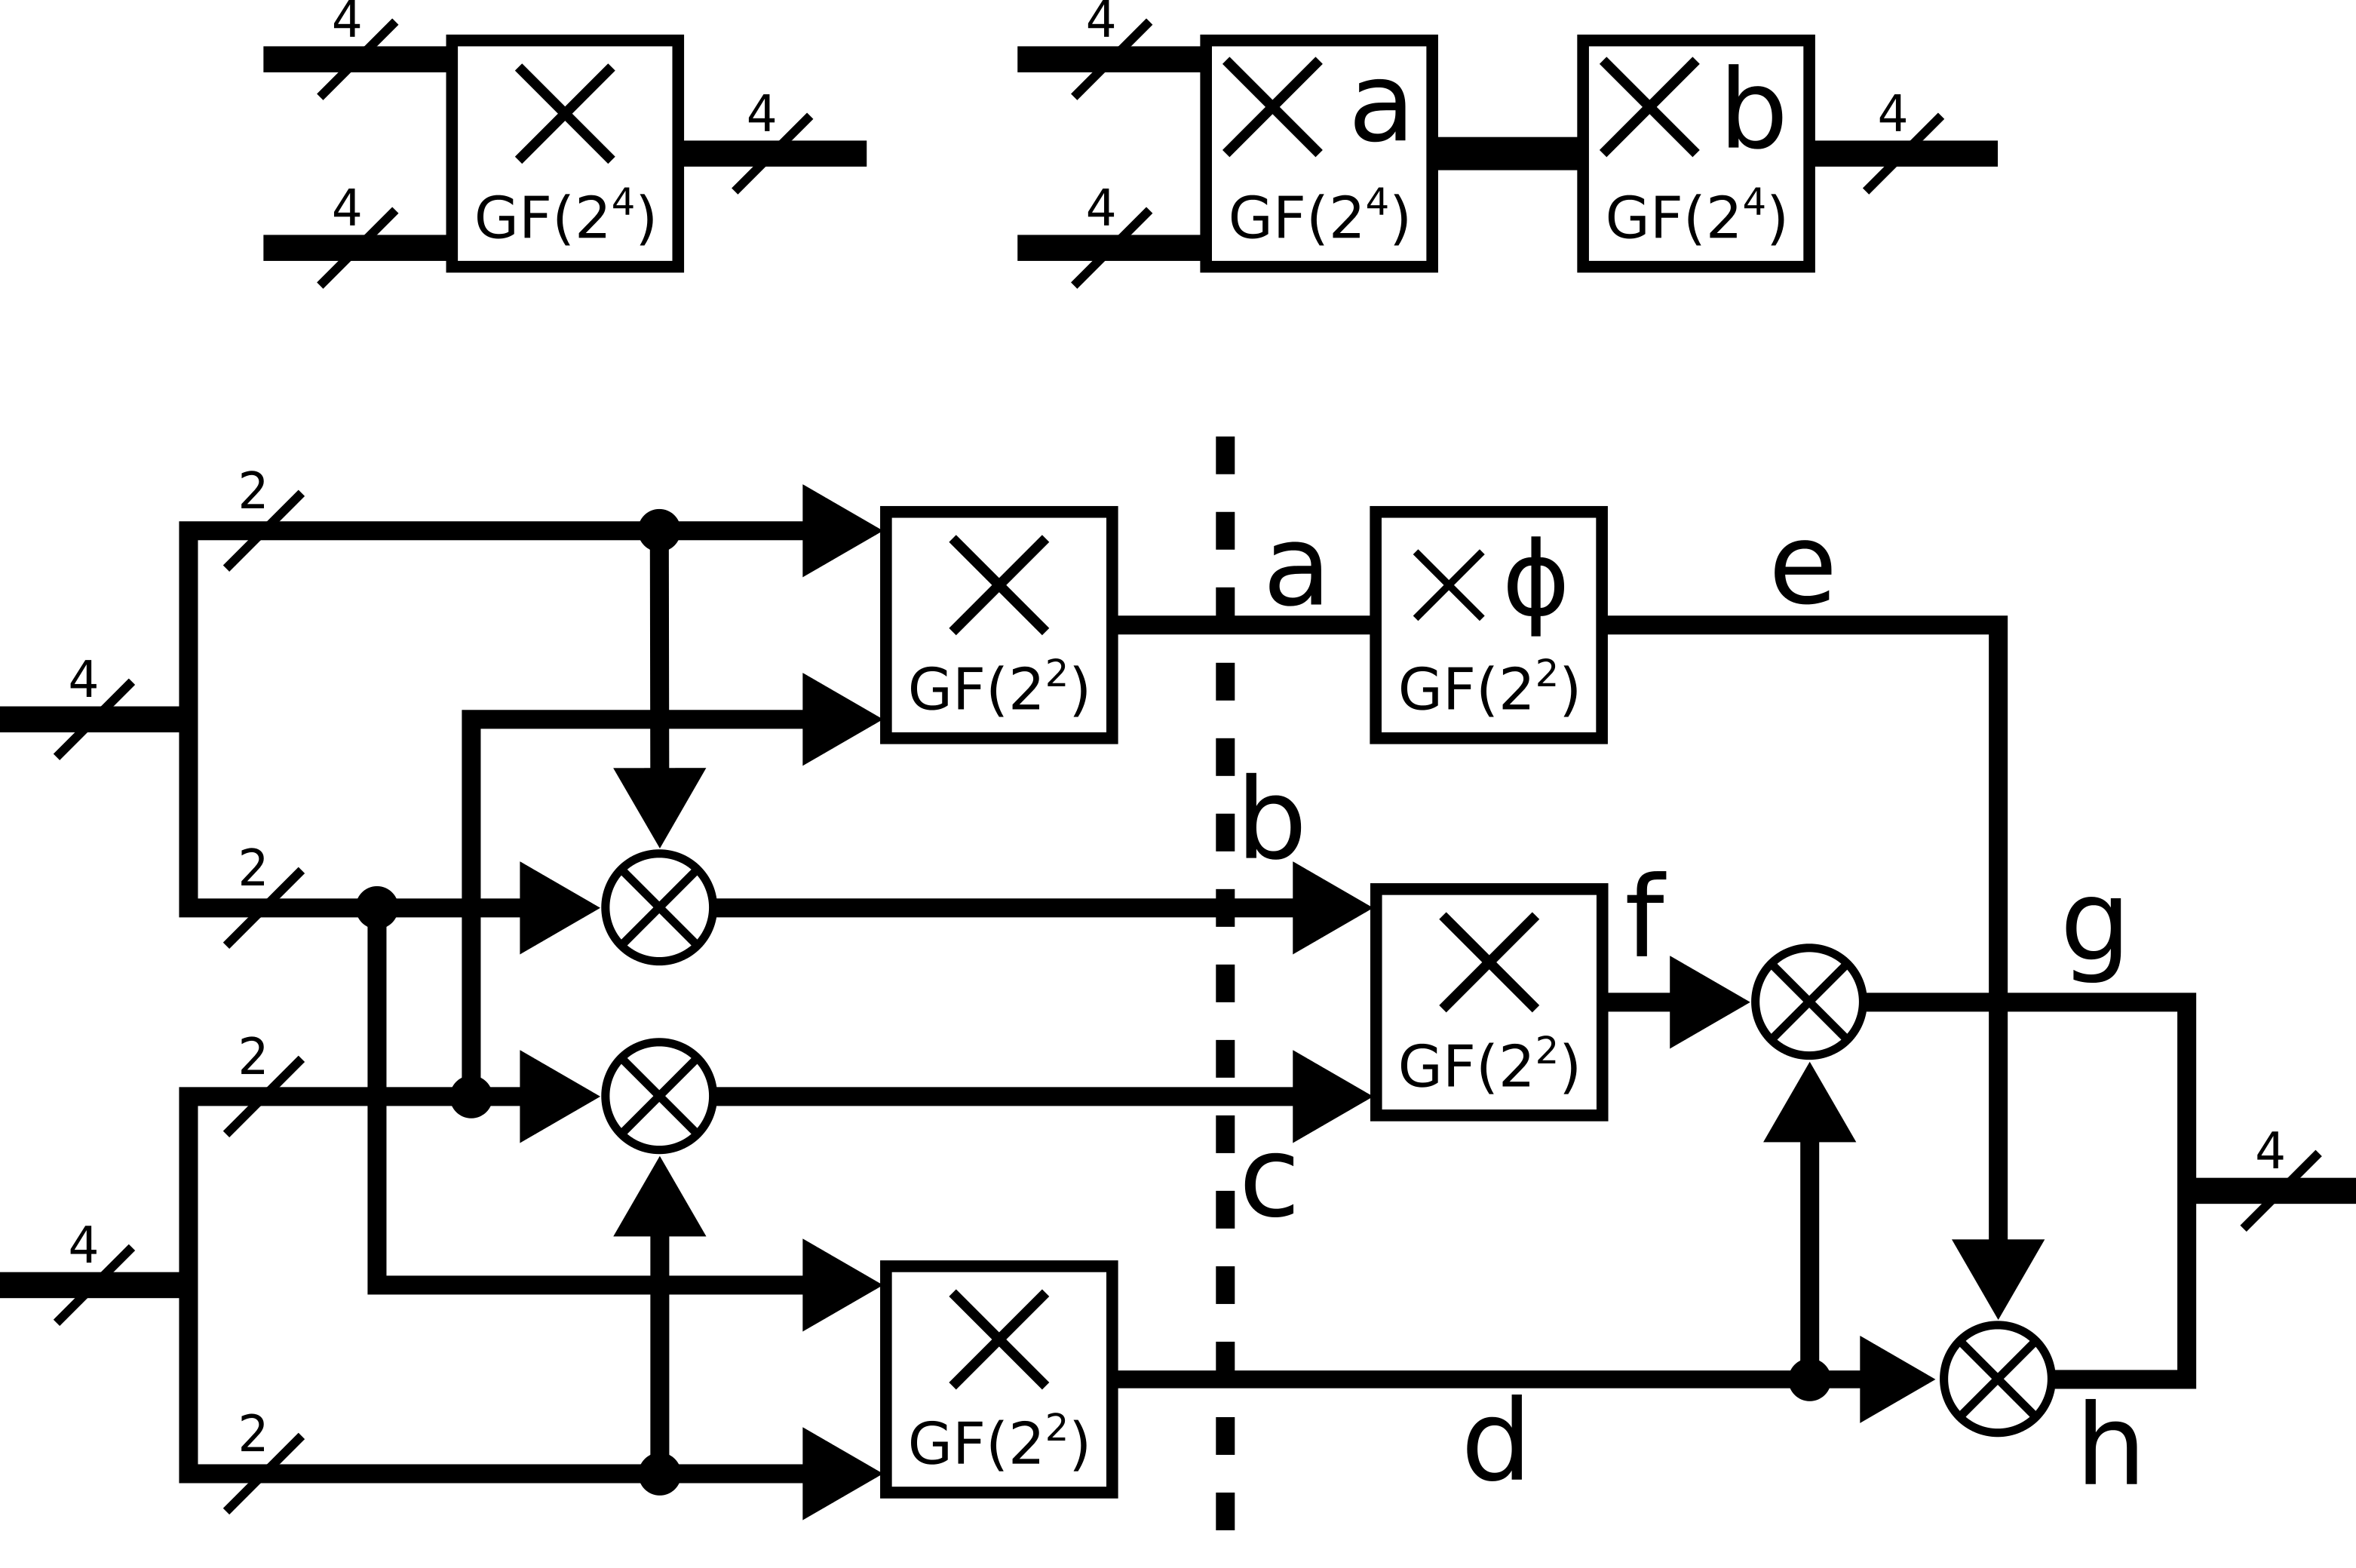
\includegraphics[scale=4]{mul-gf4-split}
\caption{Decomposition of multiplication in $GF(2^4)$ into two stages}
\label{fig:mul-gf4-split}
\end{figure}

This split uses only 4-input LUT operation mode, because:
\begin{itemize}[nolistsep]
\item Each bit of signals $a$ and $d$ depends on no more than 3 input signals, because on their paths there are only multiplications in $GF(2^2)$, which have this property. 
\item Each bit of signals $b$ and $c$ depends only on 2 input signals, because they are xors.
\item Each bit of signal $e$ depends on no more than 2 input signals, because this is a property of multiplication by $\phi$.
\item Each bit of signal $f$ depends on no more than 3 input signals, because this is a property of multiplication in $GF(2^2)$.
\item Each bit of signal $g$ depends on no more than 4 input signals, because signals from $f$ are xored with independent signals.
\item Each bit of signal $h$ depends on no more than 3 input signals, because signals from $e$ are xored with independent signals.
\end{itemize}


\paragraph{Squaring in $GF(2^4)$}\mbox{}\\
This operation has only 4 inputs, so it is can already be implemented using a 4-input LUT.


\paragraph{ShiftRows transformation}\mbox{}\\
This transformation does not do combinatorial logic and thus can be joined with any other operation to form a stage.


\paragraph{MixColumns transformation}\mbox{}\\
Lets first notice that some output bits of multiplication by $\{02\}_{16}$ depend on 2 input signals (\ref{eq:mul2}). In MixColumns transformation this multiplication is performed on signals which were are already $xored$ (fig. \ref{fig:mix_columns}). This means that outputs of multiplication by $\{02\}_{16}$ blocks already depend on $2 * 2 = 4$ signals. Those outputs are then xored again, which results in exceeding 4-input limit. MixColumns transformation, therefore, needs to be split into two stages. It can be done as shown in figure \ref{fig:mix-columns-split}.

\begin{figure}[!h]
\centering
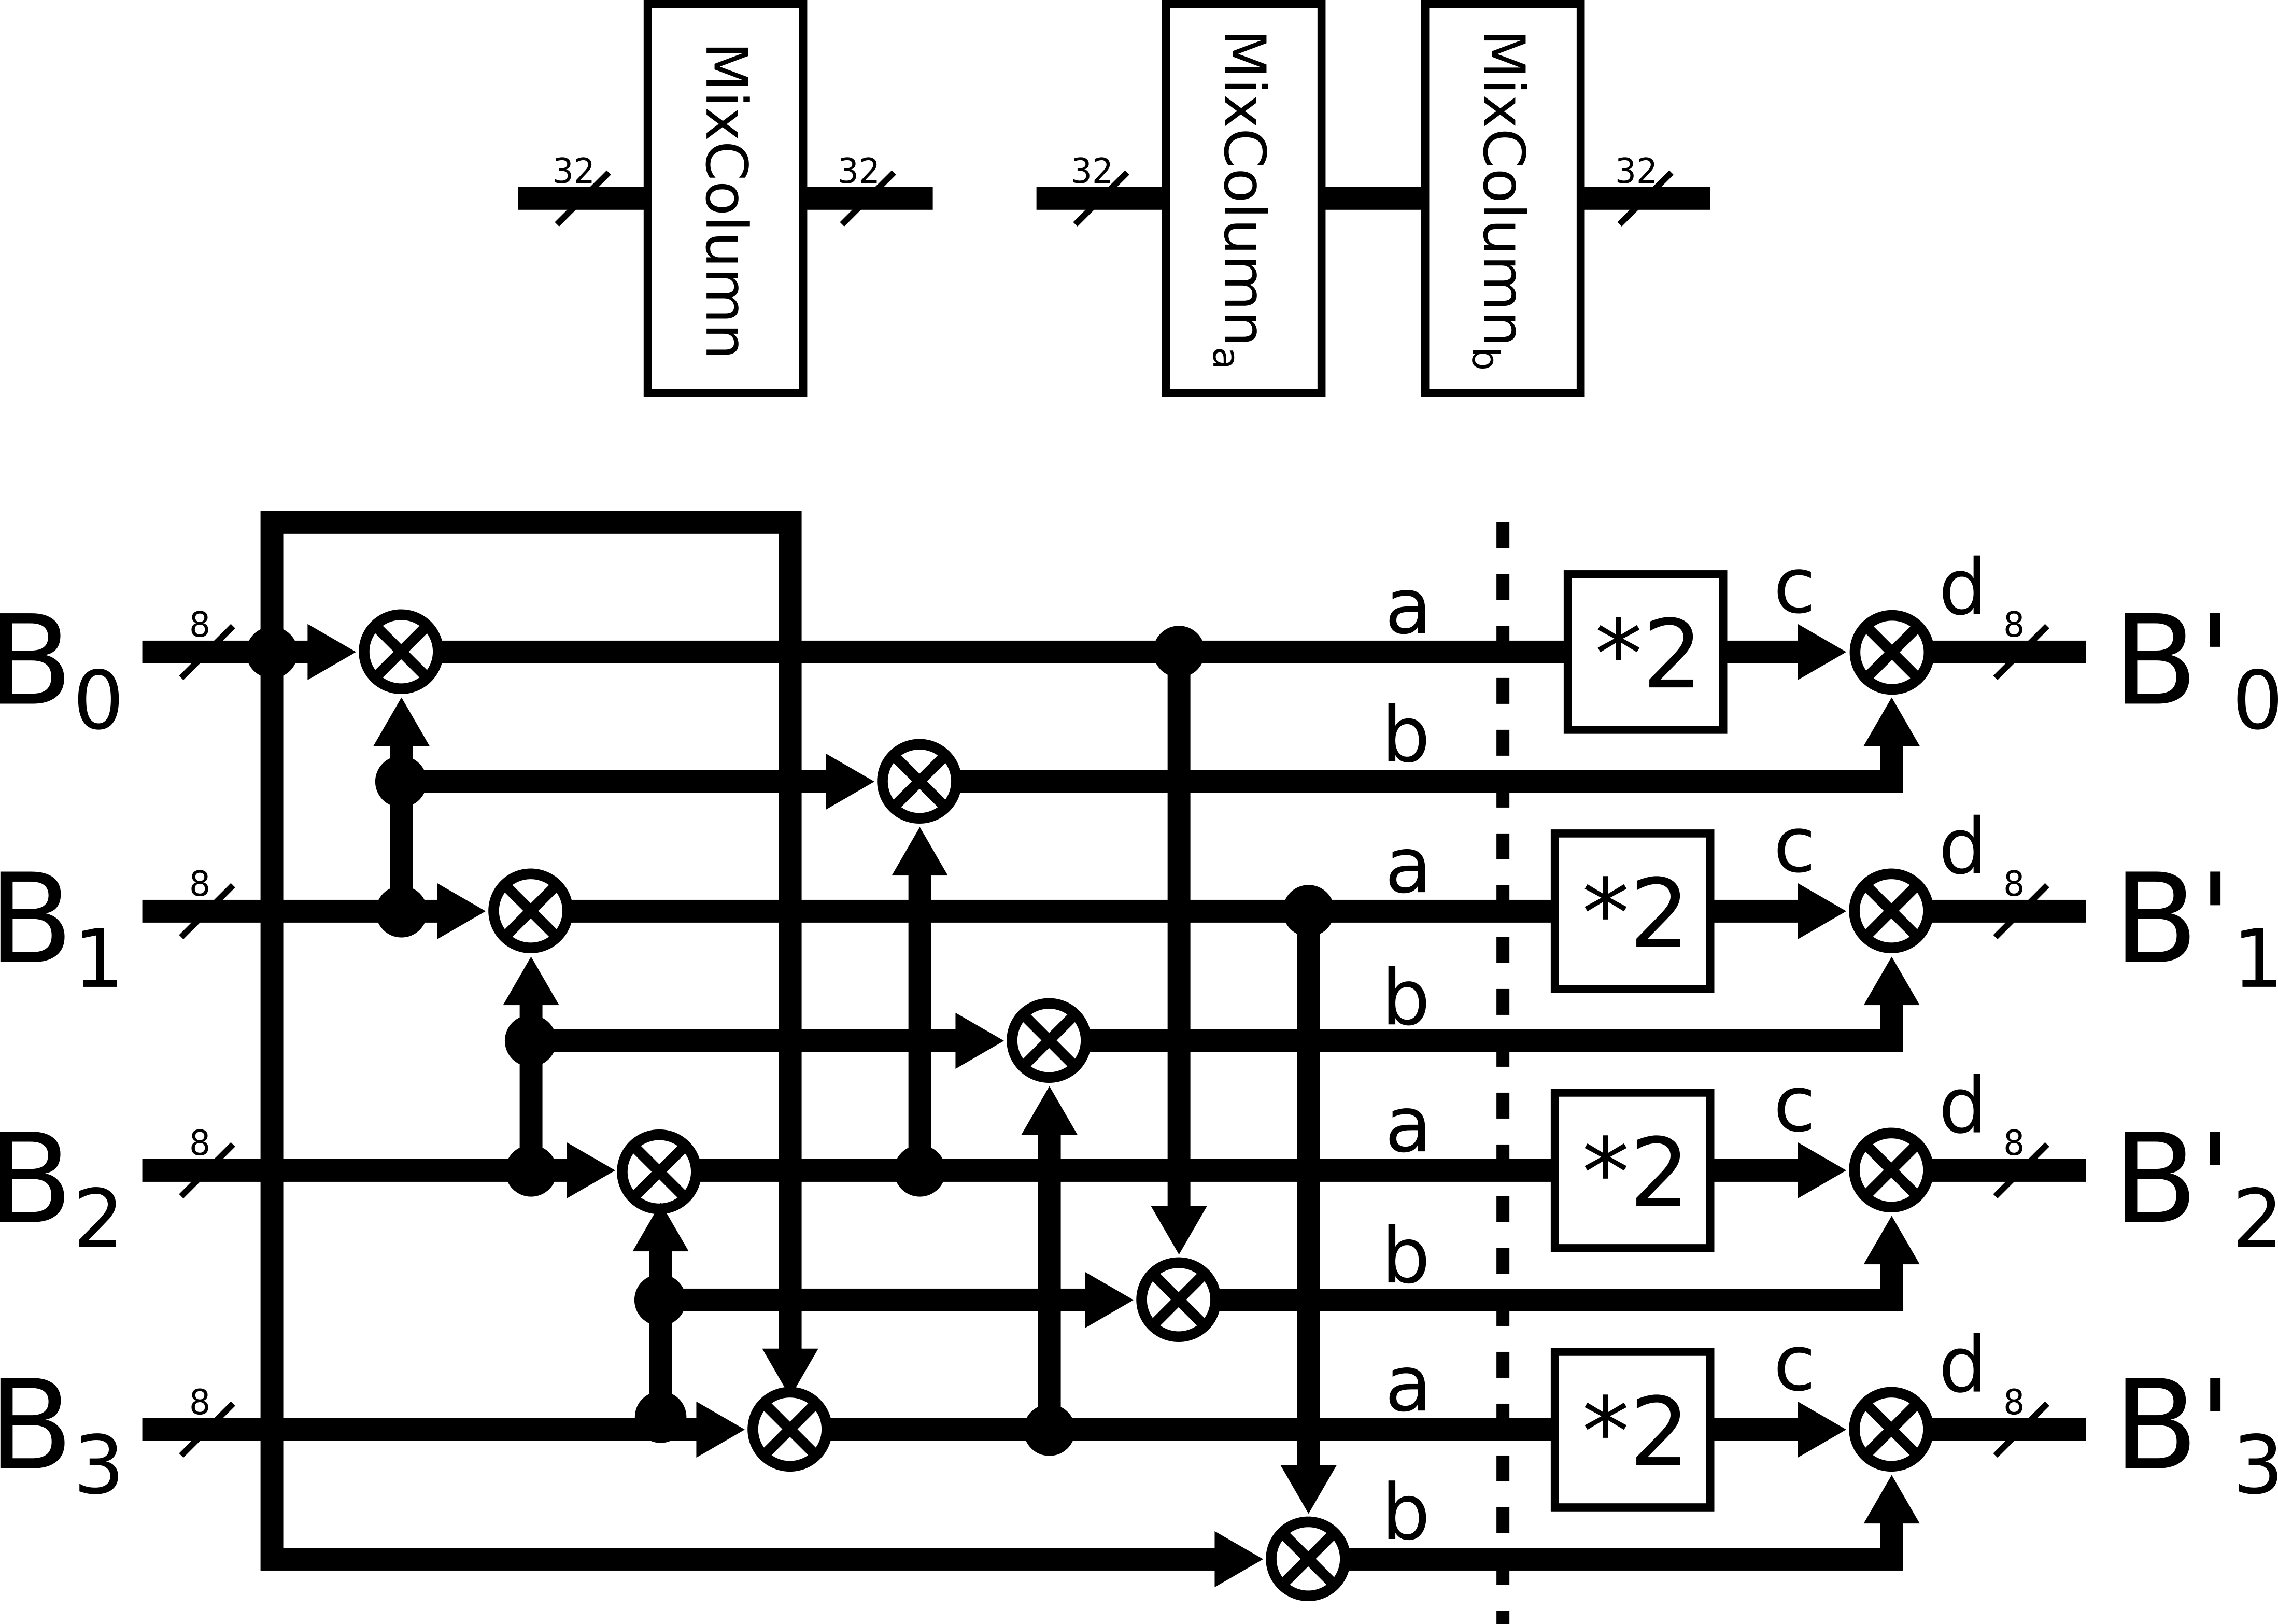
\includegraphics[scale=3]{mix-columns-split}
\caption{Decomposition of MixColumns transformation into two stages}
\label{fig:mix-columns-split}
\end{figure}

Those stages can be implemented using only 4-input LUTs, because:
\begin{itemize}[nolistsep]
\item Each bit of signals marked $a$ depends on 2 input signals.
\item Each bit of signals marked $b$ depends on 3 input signals.
\item Each bit of signals marked $c$ depends on no nore than 2 input signals.
\item Each bit of signals marked $d$ depends on no nore than 3 input signals.
\end{itemize}

Note that all output bits depend on no more than 3 input signals, which means that they can be $xored$ with other independent inputs in one stage. This is useful for combining it with AddRoundKey transformation.


\paragraph{AddRoundKey transformation}\mbox{}\\
This transformation consists only of a xor gate, which means that it can be combined into one stage with MixColumns.


\paragraph{$Rot$ operaiton in KeyExpansion}\mbox{}\\
$Rot$ operation rotates a word (4 bytes) left by one byte, therefore it does not require any combinatorial logic. Similarly to ShiftRows transformation it can be joined with any other operation to form a stage.

\paragraph{$Rcon$ operation in KeyExpansion}\mbox{}\\
$Rcon$ operation xors highest byte of a word with $2^{N + 1}$, which means that it adds at most one signal to input. It is performed after second stage of mapping $f^{-1}(x)$ from $GF((2^4)^2)$ to $GF(2^8)$ combined with AES affine transformation ($f_b^{-1}(x)$), outputs of which depend on only 2 input bits. This means that combining $f_b^{-1}(x)$ with $Rcon$ in a stage results in outputs depending on 3 bits, which still leaves space in this stage. This one extra signal is utilised in KeyExpansion pipeline.

\paragraph{Final design of throughput-optimized AES encryption circuit}\mbox{}\\
Taking all points presented in this section into consideration, it follows that a pipelied circuit using only 4-input LUTs can be implemeted according to diagram in figure \ref{fig:high-speed-pipe-full}.



